% -*- root: Document.tex -*-

\section{Container and Node Profiling}
\label{sec:monitoring}

System containers can exhibit a wide diversity of properties and requirements, from CPU-intensive tasks running for a short duration to longstanding memory-intensive applications serving user requests.
In such a context where the workloads are unknown, it is particularly challenging to ensure an efficient scheduling of these containers.
We therefore propose to introduce a resource profiling phase within \GP{} to automatically learn the resource requirements of a container during the beginning of its execution, and to subsequently use this information to compute a resource envelope that will help the \GP{} scheduler to appropriately place the container on the best fitting node for the rest of its execution.
In particular, this container profiling phase is performed within the \emph{nursery} and \emph{young} generations of \GP{} and is complemented with a monitoring of the nodes located in the \emph{young} and \emph{old} generations in order to maintain a up-to-date cartography of available resources in the cloud data center.

\paragraph{Profiling the resources consumption.}

Upon deployment of a new container within the \emph{nursery} generation, \GP{} uses a \textsc{cAdvisor} daemon~\cite{cAdvisor} to collect, aggregate, process, and export metrics about running containers every $30$ seconds.
In particular, \textsc{cAdvisor} logs resource isolation parameters, historical resource usage, histograms of complete historical resource usage, and network statistics for each system container running on a \textsc{Docker} host.
Collected metrics are automatically exported towards an \textsc{InfluxDB} service~\cite{influxdb} hosted on the master node (see Figure~\ref{fig:monitoring}).
\textsc{InfluxDB} provides a time-series database to store cluster-wide metrics per container, according to a specific data retention policy ($x$ minutes in \GP{}).
Whenever needed, \GP{} can therefore query \textsc{InfluxDB} to learn about the containers' workloads.

\begin{figure}[t]
\centering
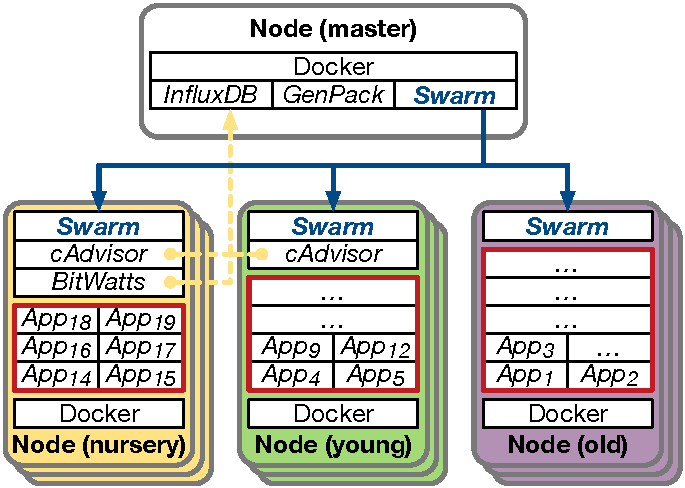
\includegraphics[width=.7\linewidth]{figures/monitoring}
\caption{Overview of the monitoring support in \GP{}.}
\label{fig:monitoring}
\end{figure}

\paragraph{Computing the container envelopes.}

Periodically, \GP{} picks the containers running in the \emph{nursery} generation and triggers a scheduling phase for all of them.
As part of this phase, \GP{} queries \textsc{InfluxDB} to convert raw resource metrics into \emph{container envelopes}, which will be used by the scheduler to estimate the expected resource consumption.
In particular, for each resource, \GP{} first computes the metrics distribution and extracts the \emph{$90^{\,th}$ percentile} value as a component of the resource envelope.
Then, \GP{} splits the set of containers into $k$ clusters by applying the \emph{k-means} algorithm, which belongs to the category of unsupervised learning approaches.
For example, we can set $k=4$ to segregate $4$ classes of CPU-, disk-, network-, and memory-intensive workloads into $4$ container envelopes.
% \cf{Intuitively this makes sense but is there some empirical evidence that k=4 is a good choice?}

Finally, within each envelope, containers are ordered per decreasing resource consumption score, which is computed for each enclosed container~$i$ as:
\small
\[score_i=\sqrt{(\frac{cpu_i}{\sum{cpu}})^2+(\frac{disk_i}{\sum{disk}})^2+(\frac{net_i}{\sum{net}})^2+(\frac{mem_i}{\sum{mem}})^2}\,.\]
\normalsize

The resulting container envelopes are posted to the \GP{} scheduler, which is in charge of placing the containers among the nodes of the \emph{young} generation.

\begin{figure}[t!]
	\centering
	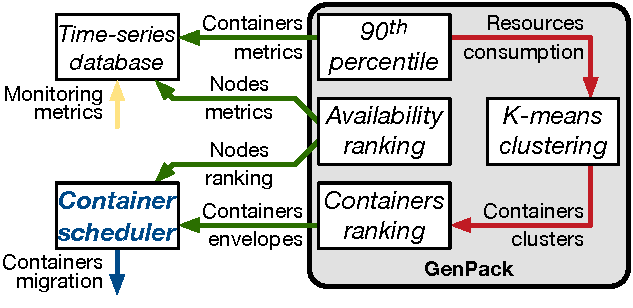
\includegraphics[width=.7\linewidth]{figures/profiling}
	\caption{Container and node profiling in \GP{}.}
	\label{fig:profiling}
\end{figure}

Beyond this first scheduling phase, \GP keeps monitoring and profiling the containers within the \emph{young} generation in order to consolidate the resource envelope prior to a later migration in the \emph{old generation}.

\paragraph{Maintaining the node availability cartography.}

\GP{} monitors the resource availability of nodes within the \emph{young} and \emph{old} generations.
For each generation, it uses this information to rank the nodes according to resource availability, least available nodes first, by computing for each node $j$ the availability level as:
\small
\[availability_j=\sqrt{cpu_{ratio}^2+disk_{ratio}^2+net_{ratio}^2+mem_{ratio}^2}\,,\]
\normalsize
\noindent which corresponds to the norm of the resource vector
$\vec{r_j}=\begin{matrix}(cpu_{ratio} & disk_{ratio} & net_{ratio} & mem_{ratio})\end{matrix}$
that \GP{} extracts from \textsc{InfluxDB}.
This ranking of nodes will then be used by the scheduler to find the first fitting node to host a container, ultimately minimizing the number of hosts to be used---\emph{i.e.}, that need to be powered up.
